\documentclass[tikz,border=10pt]{standalone}
\usepackage{amsmath,amssymb}
\usepackage{newpxtext,newpxmath}
\usetikzlibrary{arrows.meta,positioning,calc,backgrounds}

\definecolor{inkDark}{HTML}{1E293B}
\definecolor{slateSub}{HTML}{334155}
\definecolor{pathBlue}{HTML}{005A9C}
\definecolor{accentRed}{HTML}{B91C1C}
\definecolor{accentTeal}{HTML}{0E6251}
\definecolor{accentAmber}{HTML}{B45309}
\definecolor{bandBlue}{HTML}{EFF6FF}
\definecolor{bandAmber}{HTML}{FFFBEB}
\definecolor{boxFill}{HTML}{FFFFFF}

\begin{document}
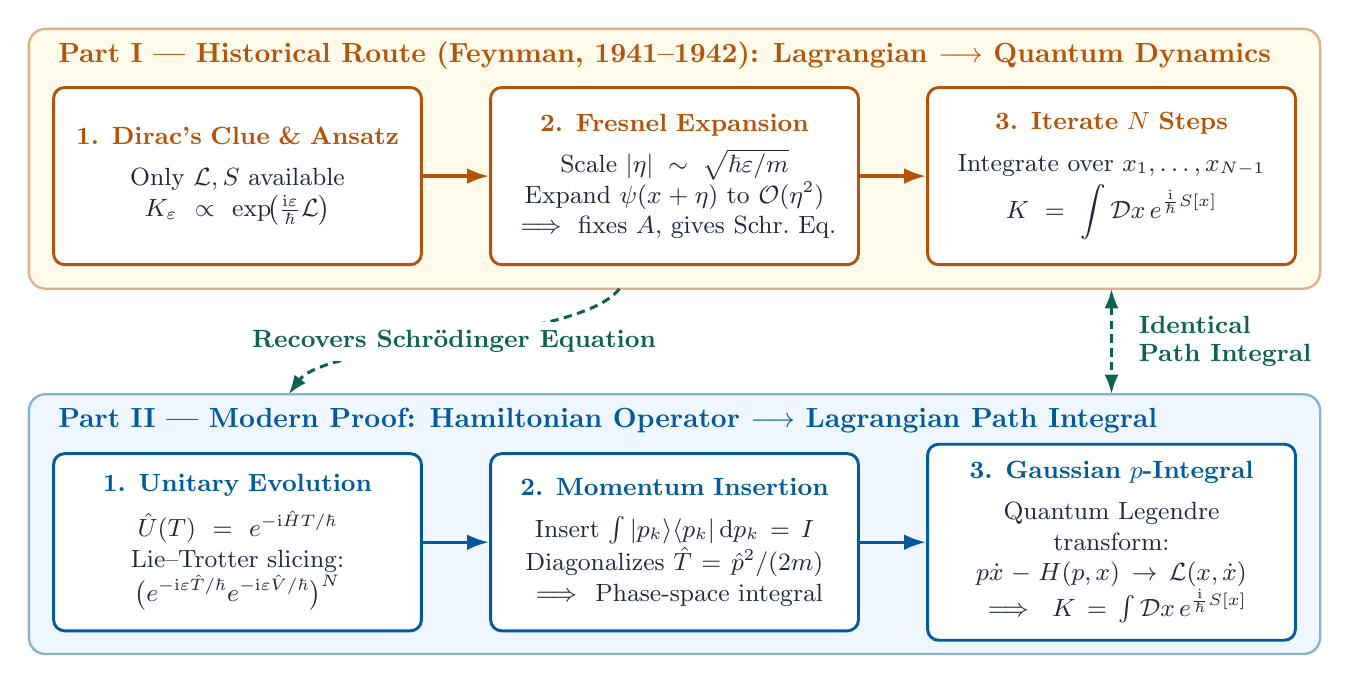
\begin{tikzpicture}[
    >=Latex,
    every node/.style={text=inkDark},
    boxHist/.style={
        draw=accentAmber, line width=1.05pt, rounded corners=4pt,
        fill=boxFill, text width=4.25cm, minimum height=2.25cm,
        align=center, inner sep=6pt, font=\small
    },
    boxMod/.style={
        draw=pathBlue, line width=1.05pt, rounded corners=4pt,
        fill=boxFill, text width=4.25cm, minimum height=2.25cm,
        align=center, inner sep=6pt, font=\small
    },
    arrHist/.style={-{Latex[length=2.8mm,width=2.0mm]}, line width=1.25pt, draw=accentAmber},
    arrMod/.style={-{Latex[length=2.8mm,width=2.0mm]}, line width=1.25pt, draw=pathBlue},
    arrEq/.style={{Latex[length=2.5mm,width=1.8mm]}-{Latex[length=2.5mm,width=1.8mm]}, line width=1.15pt, draw=accentTeal, densely dashed}
]

    % =========================================================
    % Track I: Historical Route (Feynman 1941-1942)
    % =========================================================
    \node[boxHist] (H1) at (0, 4.65) {
        {\bfseries\color{accentAmber} 1. Dirac's Clue \& Ansatz}\\[4pt]
        Only $\mathcal{L}, S$ available\\
        $K_\varepsilon \propto \exp\!\bigl(\tfrac{\mathrm{i}\varepsilon}{\hbar}\mathcal{L}\bigr)$
    };

    \node[boxHist] (H2) at (5.55, 4.65) {
        {\bfseries\color{accentAmber} 2. Fresnel Expansion}\\[4pt]
        Scale $|\eta| \sim \sqrt{\hbar\varepsilon/m}$\\
        Expand $\psi(x+\eta)$ to $\mathcal{O}(\eta^2)$\\
        $\implies$ fixes $A$, gives Schr.\ Eq.
    };

    \node[boxHist] (H3) at (11.10, 4.65) {
        {\bfseries\color{accentAmber} 3. Iterate $N$ Steps}\\[4pt]
        Integrate over $x_1,\dots,x_{N-1}$\\[2pt]
        $K = \displaystyle\int\mathcal{D}x\,e^{\frac{\mathrm{i}}{\hbar}S[x]}$
    };

    \draw[arrHist] (H1.east) -- (H2.west);
    \draw[arrHist] (H2.east) -- (H3.west);

    % =========================================================
    % Track II: Modern Textbook Proof
    % =========================================================
    \node[boxMod] (M1) at (0, 0) {
        {\bfseries\color{pathBlue} 1. Unitary Evolution}\\[4pt]
        $\hat U(T) = e^{-\mathrm{i}\hat H T/\hbar}$\\
        Lie--Trotter slicing:\\
        $\bigl(e^{-\mathrm{i}\varepsilon\hat T/\hbar}e^{-\mathrm{i}\varepsilon\hat V/\hbar}\bigr)^N$
    };

    \node[boxMod] (M2) at (5.55, 0) {
        {\bfseries\color{pathBlue} 2. Momentum Insertion}\\[4pt]
        Insert $\int |p_k\rangle\langle p_k|\,\mathrm{d}p_k = I$\\
        Diagonalizes $\hat T = \hat p^2/(2m)$\\
        $\implies$ Phase-space integral
    };

    \node[boxMod] (M3) at (11.10, 0) {
        {\bfseries\color{pathBlue} 3. Gaussian $p$-Integral}\\[4pt]
        Quantum \mbox{Legendre} transform:\\
        $p\dot x - H(p,x) \to \mathcal{L}(x,\dot x)$\\
        $\implies K = \int\mathcal{D}x\,e^{\frac{\mathrm{i}}{\hbar}S[x]}$
    };

    \draw[arrMod] (M1.east) -- (M2.west);
    \draw[arrMod] (M2.east) -- (M3.west);

    % =========================================================
    % Subtle background track bands & headers (generous clearance!)
    % =========================================================
    \begin{scope}[on background layer]
        \fill[bandAmber, rounded corners=6pt] (-2.65, 3.22) rectangle (13.75, 6.52);
        \draw[accentAmber, opacity=0.45, line width=0.85pt, rounded corners=6pt] (-2.65, 3.22) rectangle (13.75, 6.52);

        \fill[bandBlue, rounded corners=6pt] (-2.65, -1.42) rectangle (13.75, 1.88);
        \draw[pathBlue, opacity=0.45, line width=0.85pt, rounded corners=6pt] (-2.65, -1.42) rectangle (13.75, 1.88);
    \end{scope}

    \node[anchor=west, font=\bfseries\normalsize, text=accentAmber] at (-2.40, 6.18)
        {Part I — Historical Route (Feynman, 1941--1942): Lagrangian $\longrightarrow$ Quantum Dynamics};

    \node[anchor=west, font=\bfseries\normalsize, text=pathBlue] at (-2.40, 1.54)
        {Part II — Modern Proof: Hamiltonian Operator $\longrightarrow$ Lagrangian Path Integral};

    % =========================================================
    % Equivalence links placed cleanly in the open channel y in [1.9, 3.2]
    % =========================================================
    \draw[arrEq] (11.10, 3.22) -- (11.10, 1.88)
        node[midway, right=6pt, font=\small\bfseries, text=accentTeal, align=left] {Identical\\[-1pt] Path Integral};

    \draw[-{Latex[length=2.4mm,width=1.8mm]}, line width=1.1pt, draw=accentTeal, densely dashed]
        (4.85, 3.22) .. controls (4.35, 2.55) and (1.15, 2.55) .. (0.65, 1.88)
        node[pos=0.5, fill=white, inner sep=3pt, font=\small\bfseries, text=accentTeal]
        {Recovers Schr\"odinger Equation};

\end{tikzpicture}
\end{document}
